\chapter{Method}

\section{Software development methodology}

Some features of of agile software development processes, such as pair programming in Extreme Programming \cite{xpparr} and meetings in Scrum \cite{schwaber2004agile}, are only relevant to the developing software in teams, making them difficult to apply to this solo effort.

However, other principles are clearly applicable, such as valuing working software over other measures of progress such as comprehensive documentation \cite{schwaber2004agile}. Before the project began, Artoo was aleady working software, so it was important not to break it.

Another consideration is the role of the product owner, typically a customer or boss. This might have been Dr Paul Andrews, the original developer of Artoo. The lack of a formally appointed product owner to arbitrate over the requirements may have made the outcomes of this project less useful.

Gerald Jay Sussman gave a talk\footnote{\url{https://vimeo.com/12060509}} entitled ``Why programming is a good medium for expressing poorly understood and sloppily formulated ideas'' (also the title of a much earlier paper by \citet{67poorslop}).
From the claim made in this title, one can draw an indirect conclusion that a development process should be iterative, and should overlap heavily with the ``knowledge gathering'' process.
\citet{eades84} alludes to having followed this kind of process: ``Experience
shows that Hooke's Law (linear) springs are too strong when the vertices are far
apart; the logarithmic force solves this problem''; presumably, it was by implementing his algorithm using Hooke's law that \citeauthor{eades84} learned this.


\section{The structure of Artoo}

Artoo consists of some separate parts:

\begin{description}

\item[{\tt SVGGraph}] A representation of a domain graph -- not necessarily a GSN argument.
This consists of SVG shapes, most of which are graph nodes containing textual labels in the form of SVG {\tt ForeignObject}s; and SVG paths representing the graph's directed edges.
The shapes can be moved around the canvas by clicking and dragging, and the edges appear as automatically drawn quadratic B\'{e}zier curves. 

Although this abstraction is described as ''general SVG graph tool code'', the scope of the features included in it appears to anticipate GSN-specific use. Clear examples of this are the ability to attach diamonds to shapes (which can representing undeveloped parts of the argument), the notion of connections being either horizontal (anticipating the GSN's InContextOf relationship) or vertical, and the particular SVG shapes on offer (rectangle, rounded rectangle, rhomboid, ellipse, etc. -- all happen to correspond with types of GSN element).

\item[{\tt GSNGraph}] A wrapper around {\tt SVGGraph}, containing additional methods and data structures, and applying GSN-specific terminology: for example, {\tt markNodeUndeveloped(id)} makes use of {\tt SVGGraph}'s {\tt addDiamondToShape(id)} method, but also updates the `undeveloped' property of the {\tt GSNGraph}'s own representation of the node.

\end{description}
  
Alongside this is other functionality, such as the ability to export PNG images of arguments, and the user interface with menus and dialog boxes to facilitate creating GSN arguments and generally using the tool. Further description of all the source code files can be found in \texttt{README.pdf} in the archive of supplementary material.

\section{Requirements and scope}

Informed by the findings of research discussed in chapter, and the context of the existing Artoo software, some requirements can be specified.

\subsection{Software architecture}

The presence of layers of abstraction -- GSN graphs layered upon more general graphs -- might be feasibly followed through in implementation of automatic layout: first implementing a more general layout algorithm, and then  extending it to address the specific requirements of the GSN domain. However, what the practical difference would be is moot. The most prominent extra requirement of GSN argument layout is the placement of contextual elements horizontally beside their parents, but this notion of connections being either horizontal or vertical is already built into the general {\tt SVGGraph} model. The direction of relationships is also part of {\tt SVGGraph} -- supporting undirected graphs would entail an additional property to indicate that an edge's direction should be ignored. This indicates that it doesn't matter.

\subsection{Good layout}

A ranking for the importance of the advice from different sources is proposed:

\begin{enumerate}
\item Empirical studies -- the most reliable source
\item Theories of perception -- often well reasoned
\item Common heuristics described by algorithm authors -- 
\end{enumerate}

\subsection{Speed}

\citet{Miller:1968:RTM:1476589.1476628}'s recommendations have stood the test of time. 


\subsection{Functional}

Already, Artoo only works a limited set of web browsers: recent versions of 
The features added in this project will not interact with the browser in any new way -- only needing to change the position of nodes, using methods already in the code -- so it is very unlikely that there will be any problems.


\section{Experimental methodology}

\subsection{Test data}

\begin{itemize}
    \item Four graphs from \cite{aldenthesis} were obtained
    \item Additionally, one graph from \cite{gsnstandard} was used
\end{itemize}

Up to a point, GSN arguments are quite homogeneous.


\section{Springy}

Springy.js is an existing JavaScript implementation of a force directed graph drawing algorithm.
It lays out graphs by representing nodes as point charges and edges as springs. Springy.js simulates the electrostatic forces of interaction between these point charges, and the extension of the springs caused by these forces, according to Coulomb's and Hooke's laws.

\subsection{Implementing}

Springy, as distributed online\footref{fn:springy}, consists of a layout algorithm implemented in JavaScript (springy.js) along with a sample renderer for displaying a graph layout.

\begin{figure}
  \centering
  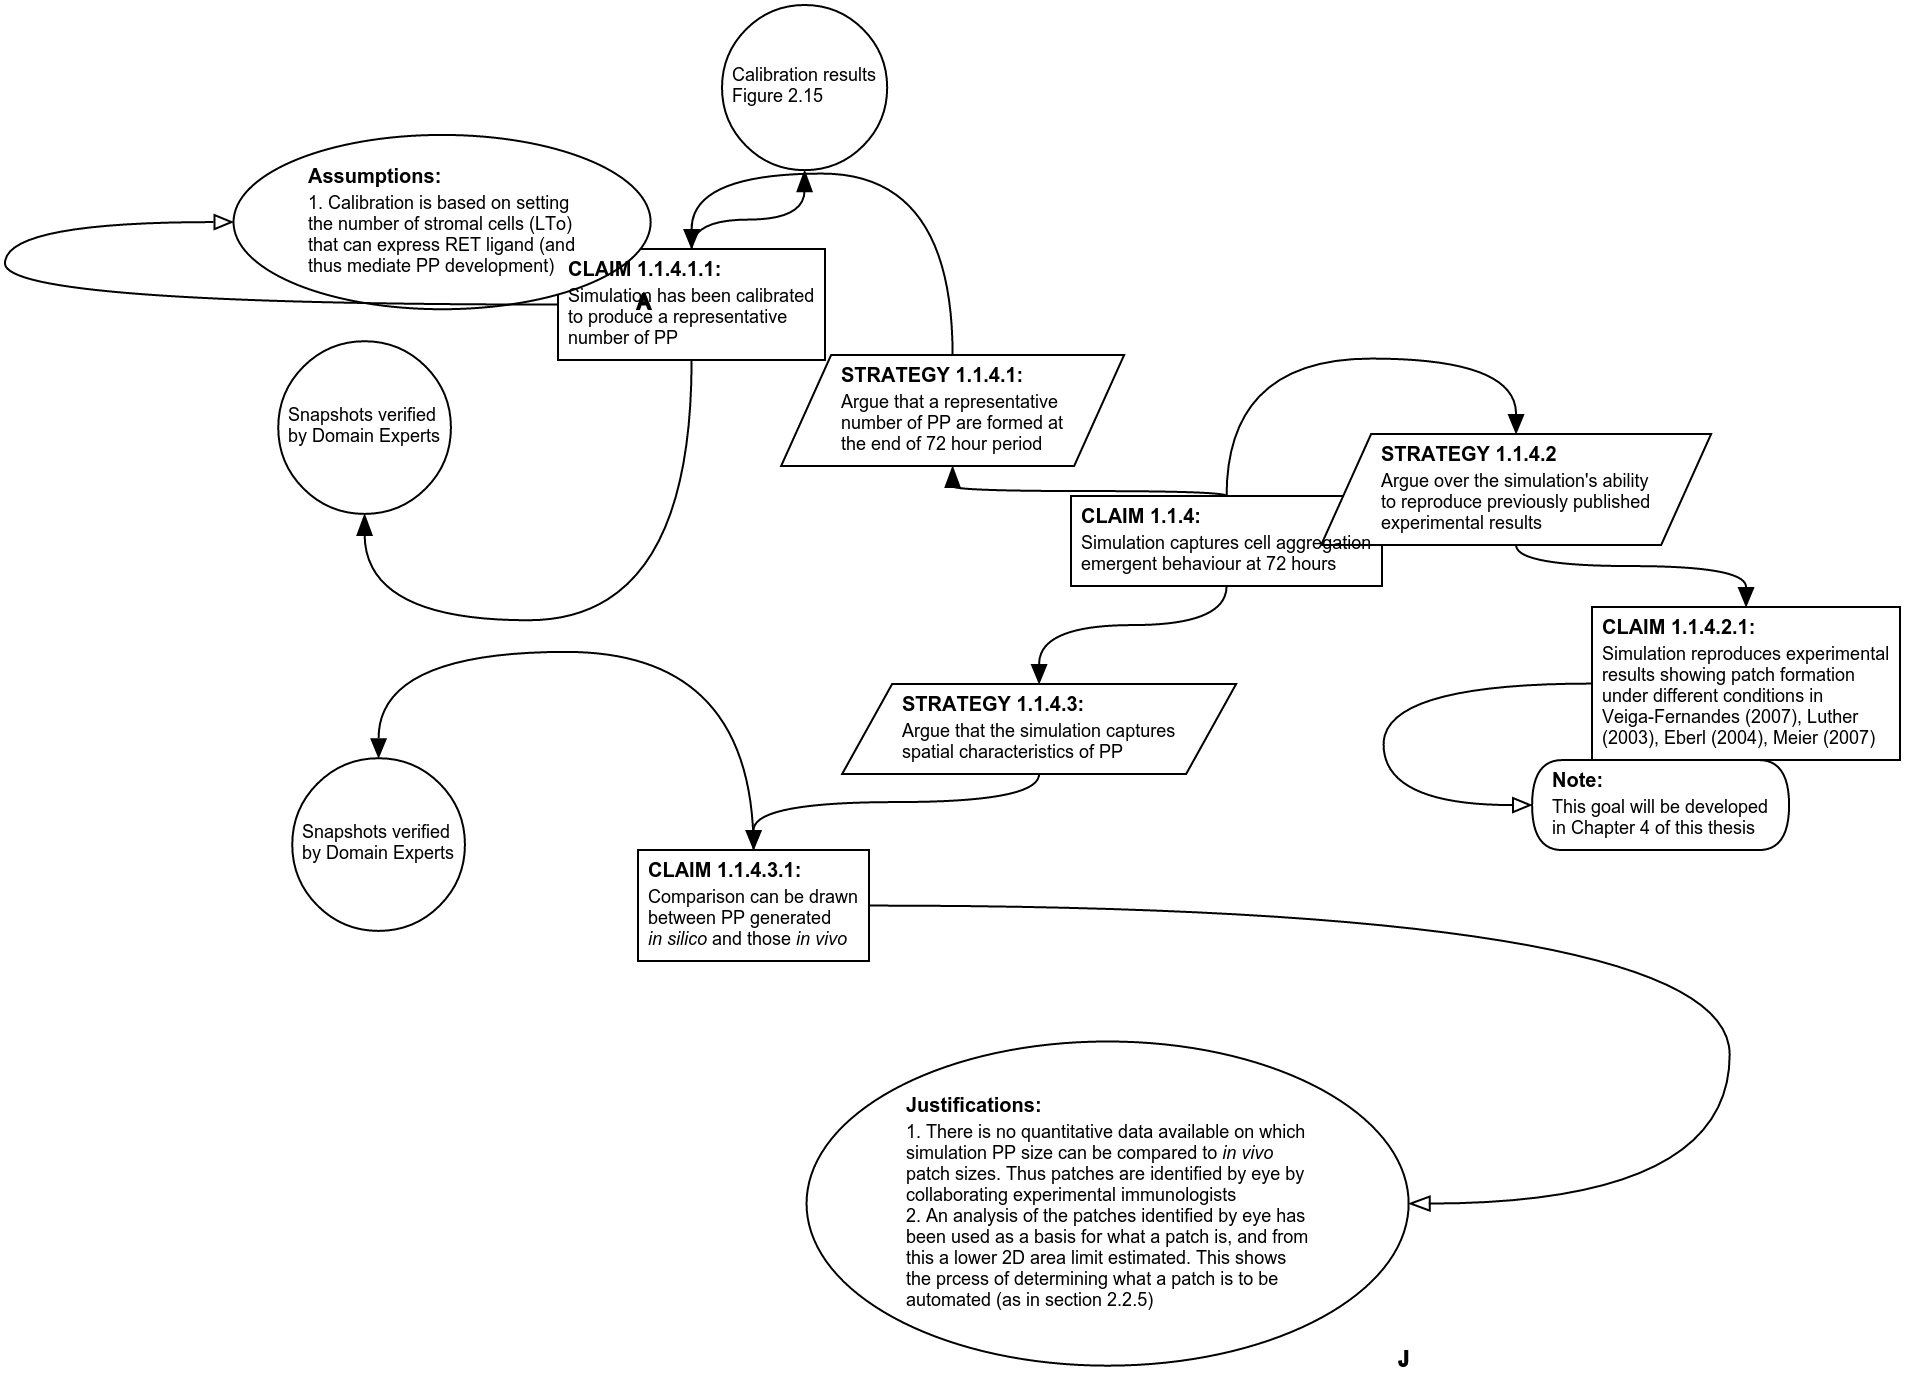
\includegraphics[width=\textwidth]{graphics/results/a4-springy.png}
  \caption{An argument laid out using Springy}
  \label{fig:dagre1}
\end{figure}


\section{Arbor}

Simple though the brute-force force directed algorithm implemented in Springy is to understand, it also inefficient. The application of the Barnes-Hut algorithm has been discussed in section~\ref{sec:forcedir}.


\section{Layered}

A key part of the layered layout approach is notion that directed graphs flow in a single direction (typically from top to bottom or from left to right). This is highly applicable to GSN arguments, particularly as specified by the GSN community standard document's guidelines \cite{gsnstandard}.

Dagre is is a third-party implementation of a robust layered graph layout algorithhm.

\begin{figure}
  \centering
  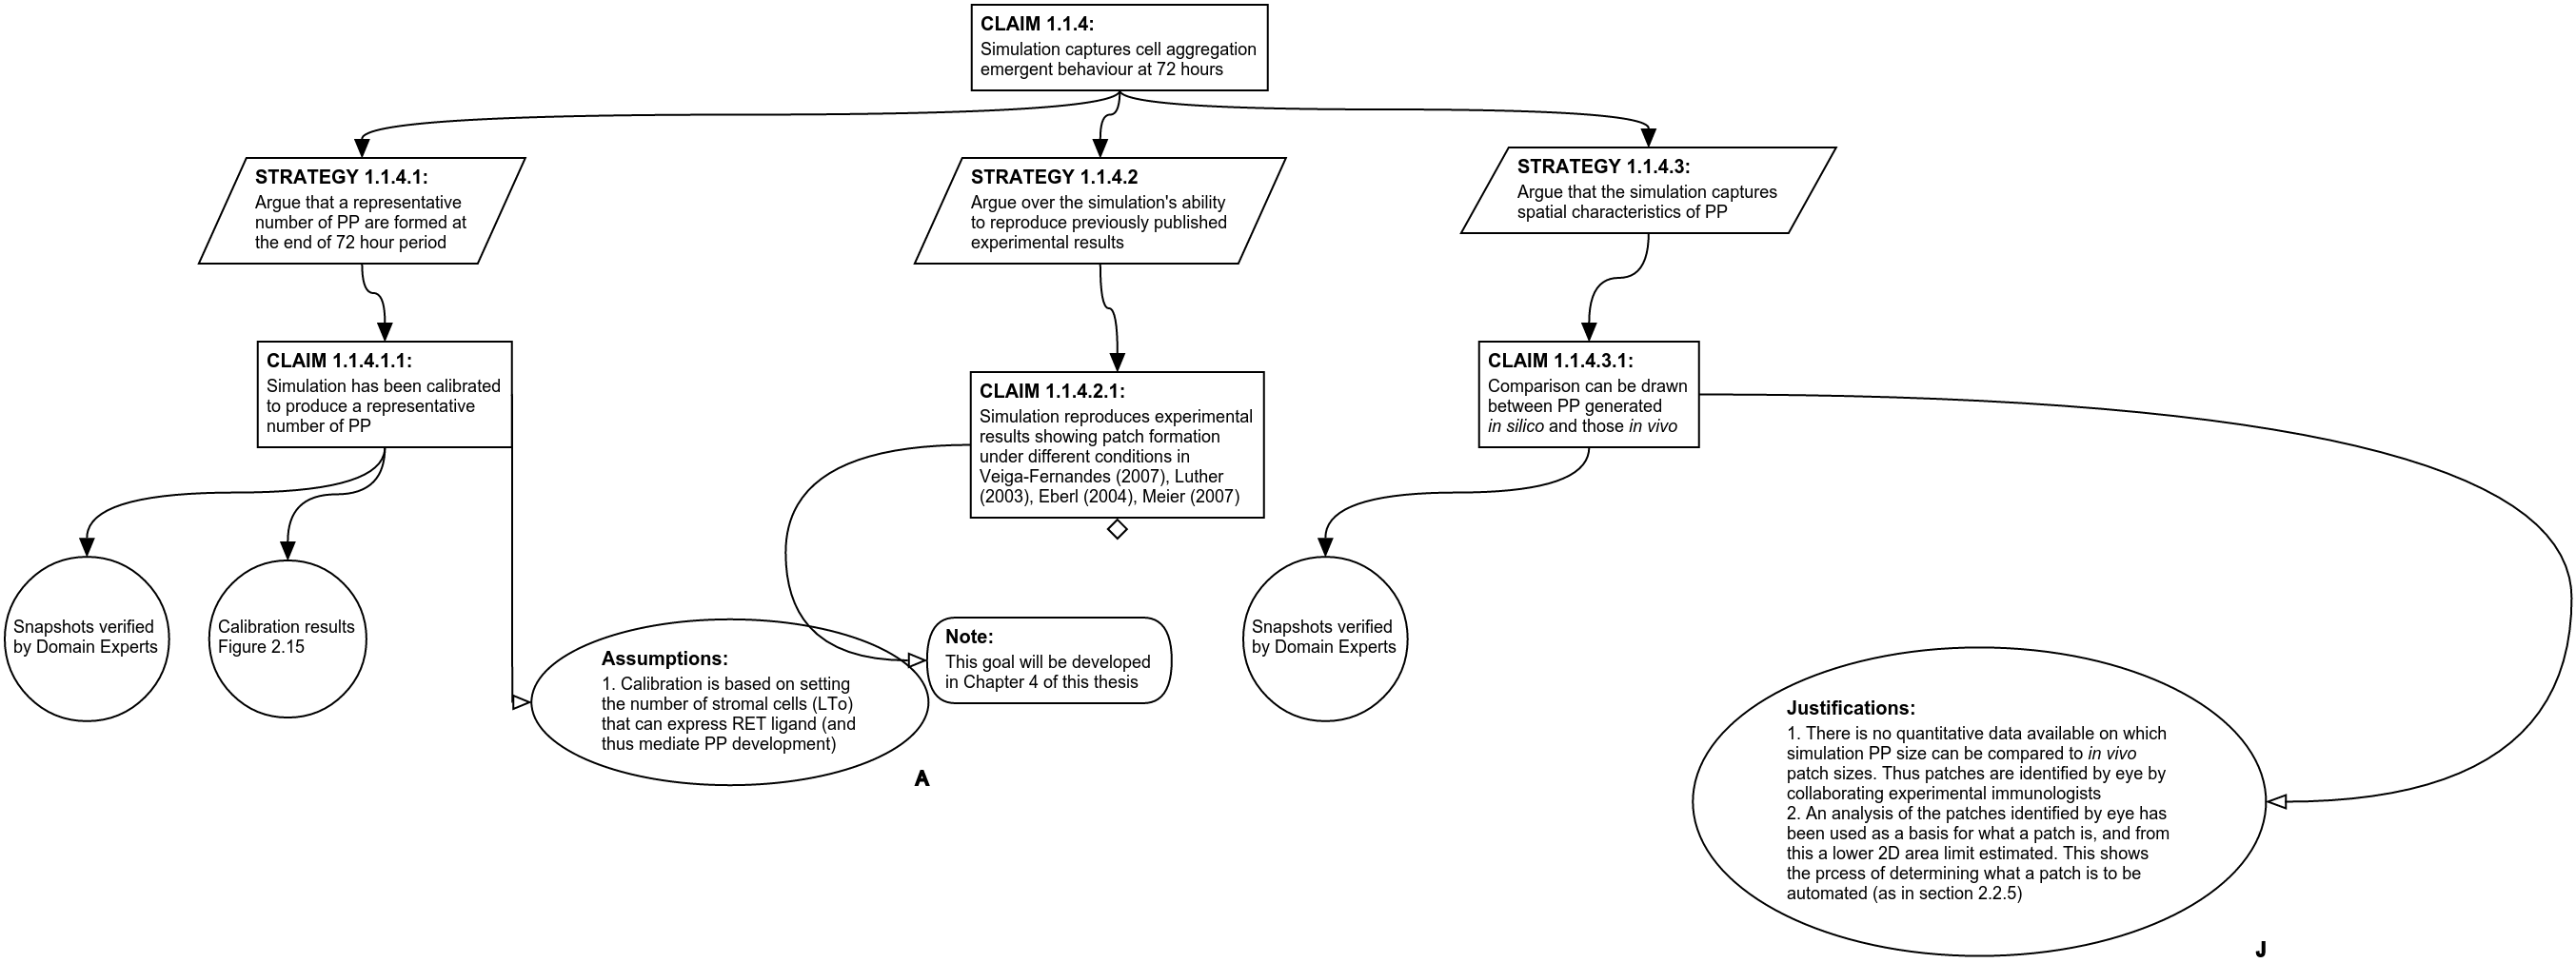
\includegraphics[width=\textwidth]{graphics/results/a4-dagre.png}
  \caption{A na\"ive use of Dagre to render a graph from \cite{aldenthesis}}
  \label{fig:dagre1}
\end{figure}

After an initial na\"ive incoproration of Dagre into Artoo, a more novel approach was begun, attempting to place context, assumption and justification elements to the sides of their parents, through the use of unrendered dummy elements,

\begin{figure}
  \centering
  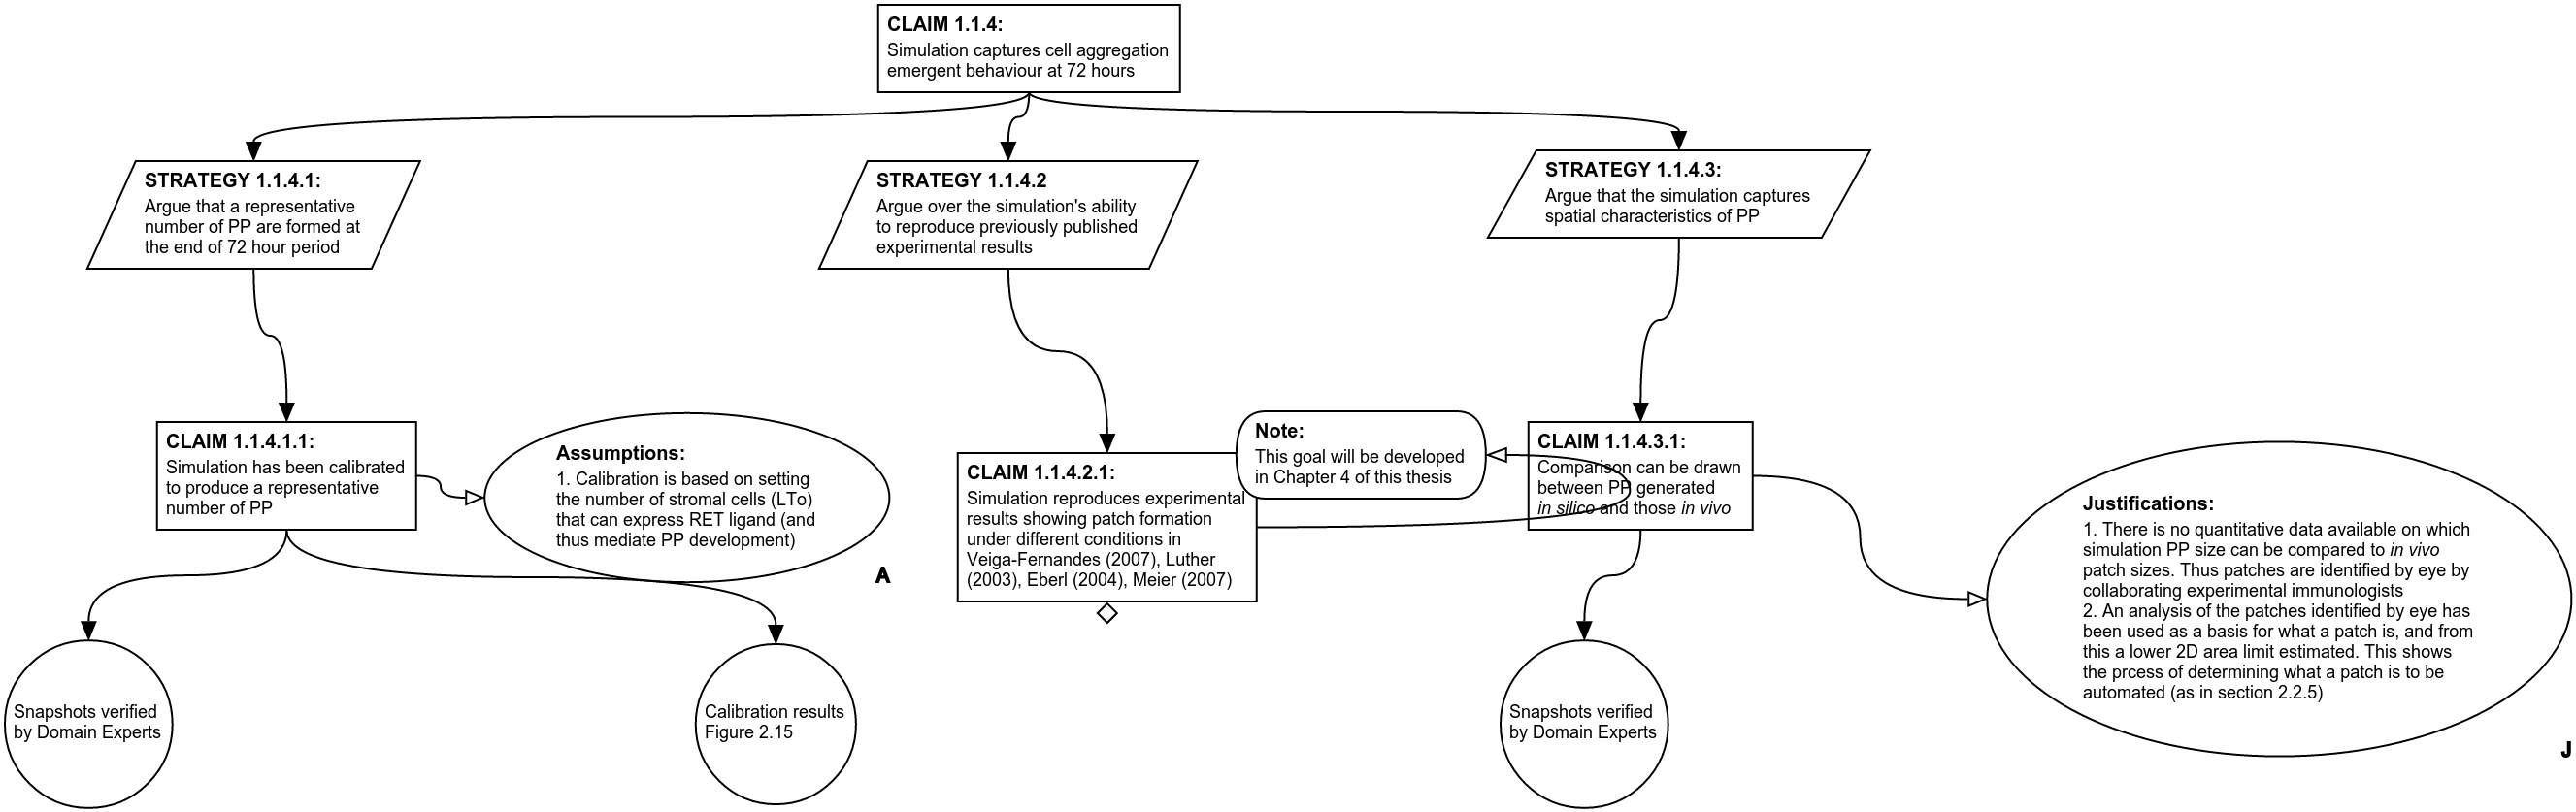
\includegraphics[width=\textwidth]{graphics/results/a4-dagre-novel.png}
  \caption{A less na\"ive use of Dagre compared to figure~\ref{fig:dagre1}, with context, assumption and justification elements placed to the sides through the use of unrendered dummy elements}
  \label{fig:dagre2}
\end{figure}


